%Document Class
\documentclass[conference]{IEEEtran}

\IEEEoverridecommandlockouts
% The preceding line is only needed to identify funding in the first footnote. If that is unneeded, please comment it out.

%Loading Packages
\usepackage{cite}
\usepackage{amsmath,amssymb,amsfonts}
\usepackage{algorithmic}
\usepackage{graphicx}
\usepackage{textcomp}
\usepackage{xcolor}

%Defining Bibtex style
\def\BibTeX{{\rm B\kern-.05em{\sc i\kern-.025em b}\kern-.08em
    T\kern-.1667em\lower.7ex\hbox{E}\kern-.125emX}}
    
%Document Begin
\begin{document}

%Paper Title
\title{Colorization Of Greyscale Images Using GANs}

%Paper Author
\author{\IEEEauthorblockN{1\textsuperscript{st} B. RaviKrishna}
\IEEEauthorblockA{\textit{Head of dept. AI\&DS} \\
\textit{Vignan Institute of}\\
\textit{Technology and Science}\\
Deshmukhi, Telangana, India \\
ravikrishnabh@gmail.com}
\and
\IEEEauthorblockN{2\textsuperscript{nd} M. Adithya Vardhan Sharma}
\IEEEauthorblockA{\textit{UG Student, dept. of CSE} \\
\textit{Vignan Institute of}\\
\textit{Technology and Science}\\
Deshmukhi, Telangana, India \\
adithyasharma1162@gmail.com}
\and
\IEEEauthorblockN{3\textsuperscript{rd} P. Bhargava Sharabha}
\IEEEauthorblockA{\textit{UG Student, dept. of CSE} \\
\textit{Vignan Institute of}\\
\textit{Technology and Science}\\
Deshmukhi, Telangana, India \\
bhargavasharabha@gmail.com\\
0009-0004-8558-7775}
}

\maketitle

%Abstract
\begin{abstract}\label{Abstract}
The process of colouring greyscale pictures has become more popular When it comes to computer vision since it allows for the conversion of monochrome photos or videos into colourful ones. This procedure is performed using deep learning algorithms, which may provide realistic and beautiful colorization. One such method is the generative adversarial network (GAN), which consists of a discriminator and a generator. While the generator learns to produce plausible and realistic colour pictures from the provided greyscale image, the discriminator draws a difference between produced and genuine colour images. The generator is trained to develop colorizations that are indistinguishable from actual pictures, while the discriminator is trained to identify manufactured images as phoney.The generator goes through this training process until it can create the most impressive and realistic colorizations. In conclusion, using deep learning algorithms to colourize grayscale pictures, like cGAN, has the potential to enhance the visual appeal of images and videos and provide viewers with a more engaging and immersive watching experience.
\end{abstract}

%Keywords
\begin{IEEEkeywords}\label{Keywords}
Colorization, Greyscale images, GAN, Generative models, Discriminative models.
\end{IEEEkeywords}

%introduction
\section{Introduction}\label{Introduction}
\IEEEPARstart{I}{n} the "colourizing" process, colour is added to black-and-white or other non-color images that are now only available in greyscale. Recent developments in computer vision and deep learning have made it possible to construct complex algorithms that can colourize grayscale pictures in a way that is both realistic and visually acceptable, which has increased the popularity of this method.

GANs are deep learning algorithms that produce exact images by modelling the distribution of a given dataset. When it comes to colorization, GANs may be trained to create realistic colour images from grayscale photos, which can then be used to produce high-quality colorizations.

A GAN used to colourize grayscale pictures primarily consists of a generator and a discriminator. The generator learns to produce convincing colour pictures from grayscale photographs while the discriminator learns to distinguish between real colour photos and artificial colour images. The generator is trained to make colour visuals that are identical to real ones in order to deceive the discriminator. Training will continue until the generator can create realistic and visually acceptable colorizations.

Utilising GANs to colourize grayscale pictures can be useful for a variety of applications, including as enhancing digital photos, recovering old photographs, and creating realistic training sets for computer vision challenges. Furthermore, given that cGANs can be trained on a variety of datasets, they may be taught to colourize a range of pictures, including objects, faces, and landscapes.

A powerful technique that has the potential to fundamentally alter image processing and restoration is GAN-based colorization of grayscale pictures. GANs might eventually supplant current techniques for colouring grayscale photos in a variety of applications with greater research and development.

%Literature Survey
\section{Literature Survey}\label{Literature Survey}
Before starting this project, we did survey on already existing systems and we looked up few research papers on already existing systems and some of them are following:

Ivana Žeger: "Grayscale Image Colorization Methods: Overview and Evaluation". The paper discusses and evaluates various techniques and approaches, particularly deep learning, used for colorizing grayscale natural photographs and the challenges involved in evaluating the quality of the resulting images. 

Yee-Hong Yang: "Automated Colorization of a Grayscale Image With Seed Points Propagation" The paper proposes a fully automatic grayscale image colorization approach using neural networks and optimization, which outperforms state-of-the-art algorithms and involves dividing grayscale photos into superpixels, extracting features of specific places of interest, propagating generated colour points to neighboring pixels, and improving the colorized image using a guided image filter.

Sonja Grgić: "An Overview of Grayscale Image Colorization Methods" The paper discusses the challenging field of automated grayscale to colour image conversion using art, machine learning, and deep learning techniques and highlights the benefits and drawbacks of various methods, with a focus on deep learning algorithms which provide high-quality and fast automatic conversion.

Swathy Titus: "Fast Colorization of Grayscale Images by Convolutional Neural Network" The paper discusses image colorization, a challenging process that involves adding chrominance values to grayscale images, and presents a convolutional neural network-based colorization approach that outperforms other methods and can be used in various contexts such as colorizing historical photographs and scientific images.

R.Shiva Shankar: "A Novel approach for Gray Scale Image Colorization using Convolutional Neural Networks" The paper discusses the use of deep learning algorithms, specifically convolutional neural networks, in the automated process of image colorization, highlighting the feature extractor and fusion layer, and showing that CNNs perform better than other methods in colorizing grayscale images.

Julien Mairal: "Sparse Representation for Color Image Restoration" The author presents an extension of the K-SVD method for sparse decomposition of signals, specifically for learning dictionaries for color images, which addresses nonhomogeneous noise and missing data, and has potential applications in color image denoising, demosaicing, and inpainting.

G. Sapiro: "Fast image and video colorization using chrominance blending" A condensed set of chrominance scribbles is delivered to the user as part of the author's straightforward and effective colorization technique, which allows users to obtain high-quality colorization results for still photos and videos with the ability to change the colours of existing colour images or videos at a fraction of the complexity and computational cost of previously described solutions.

Jorge Visca: "Image Colorization with Neural Networks" The paper proposes an automatic technique for colourizing images using a classifier trained over a set of training colour and grayscale images, which is based on back propagation and Self Organizing Maps to reduce colours and create accurate approximations for each colour in the training set.

Ishtiaq Rasool Khan: "Colorization Of Grayscale Images Using Deep Learning" The author suggests a new approach to efficiently colorize monochromatic images using a combination of deep learning and image processing, as it is a challenging and time-consuming task to perform manually using Adobe Photoshop or MATLAB.

Miao Yang: "An Underwater Color Image Quality Evaluation Metric" The author proposes a new metric, UCIQE, for evaluating underwater color image quality based on subjective testing, which takes into account the unique absorption and scattering properties of water and correlates with elements like sharpness and color in the CIELab color space; experiments demonstrate its effectiveness in real-time processing and ability to predict degradation, and its ability to perform on par with top natural color image quality metrics and underwater grayscale image quality metrics.

%Proposed System
\section{Proposed system}\label{Proposed system}
The data preparation, model architecture, training process, and colorization process are the four key parts of the proposed method for colourizing greyscale photos using GANs.

In the data pretreatment stage, the greyscale pictures are collected and prepared for the model. The photographs must now be prepared for the model, shrunk to a standard size, and have the pixel values normalised. Data sets are separated into training, validation, and testing categories.

The two core components of the model architecture are a generator network and a discriminator network. While the generator network adds colour to the grayscale images, the discriminator network distinguishes between fake and real colour images. The generator network receives the grayscale picture as an input and utilises a U-Net architecture to generate the necessary coloured image. The discriminator network, which accepts both colour and grayscale pictures and generates a binary classification score, uses convolutional neural networks (CNNs).

The generator network is trained to produce colourized images that can fool the discriminator network into classifying them as real, while the discriminator network is trained to distinguish accurately between the generated and genuine colour images. The generator and discriminator networks are jointly trained using adversarial loss during the training procedure.

In the colorization phase, fresh greyscale pictures are lastly coloured using the trained generator network. From a fresh greyscale image, the generator network generates the equivalent colour image. The colorization method enables the real-time colouring of videos and live streaming.

All things considered, the recommended technique for colourizing grayscale images with GANs is a powerful tool that can be used for a number of applications, such as image editing, video processing, and medical imaging. With more adjustments and optimisations, this method has the potential to totally transform computer vision.

%Methodology
\section{Methodology}\label{Methodology}
Ian Goodfellow and other academics introduced the generative algorithm GAN in 2014. In order to produce new samples, GAN attempts to replicate the distribution of the input dataset. GAN may be compared to a game in which two players try to discriminate between real and false notes while one player tries to make fake notes. When one player creates phoney notes that are convincing enough to lead the other player to believe they are real, GAN is said to be trained enough.

%Architecture
\subsection{Architecture}\label{Architecture}
The generative adversarial network is made up of the two smaller networks generator and discriminator. As was already established, the generator's job is to provide an output that looks exactly like genuine data. On the other hand, the discriminator's job is to determine if a sample originated from actual data or is phoney, that is, made by a generator. A multilayer perceptron model often serves as the architecture for both the generator and discriminator. 

\begin{figure}[h]
\centerline{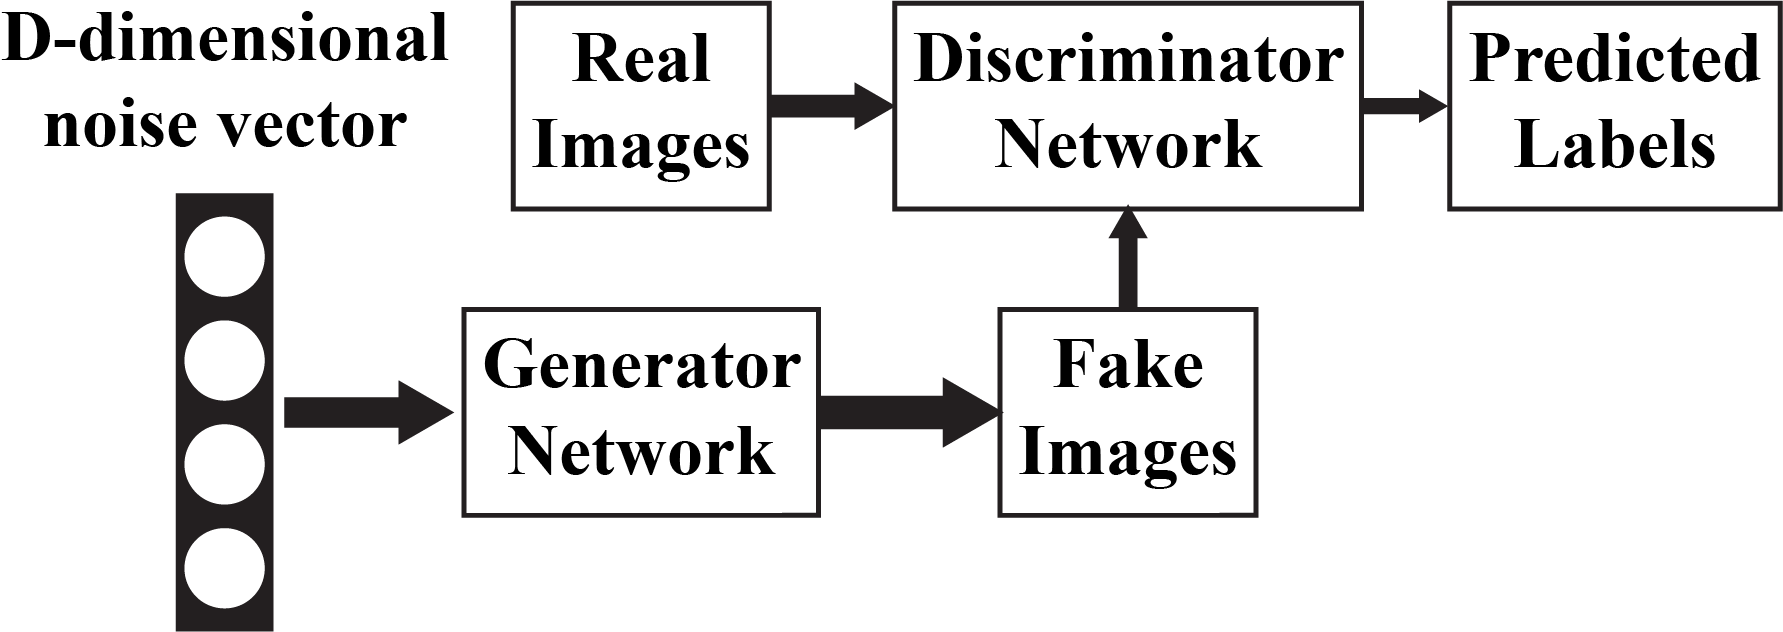
\includegraphics[width=\linewidth]{GAN-Architecture}}
\caption{GAN Architecture}
\label{fig}
\end{figure}

%Working
\subsection{Working}\label{Working}
In order to trick the discriminator, the generator creates data instances that are similar to the input dataset.$G$ therefore seeks to increase the likelihood of $D$ making a mistake. Discriminator looks for instances of fake data that the generator has produced. This framework is equivalent to a minimax two-person game, where one player is responsible for maximising the probabilities of actual images and the other for reducing the likelihood of phoney images.

%Training
\subsection{Training}\label{Training}
A generator by itself will only produce noise at random. The discriminator in a GAN theoretically directs the generator as to what data instances to produce. In order to determine what counts as actual photos, GAN constructs a discriminator. It also feeds input to the generator to aid in producing more accurate data instances.

%Training Discriminator
\subsubsection{Training Discriminator}\label{Training Discriminator}
The discriminator examines produced pictures apart from real images (training samples). It determines if the discriminator's input picture is created or real. The probability that the input x is real, or P(class of input = actual data instance), is the output $D(x)$. The discriminator is trained in the same manner as a deep network classifier. $D(x)=1$ is what we desire if the input is real. If it is produced, it ought to be zero. The discriminator finds characteristics that contribute to actual data instances through this method.

\begin{figure}[h]
\centerline{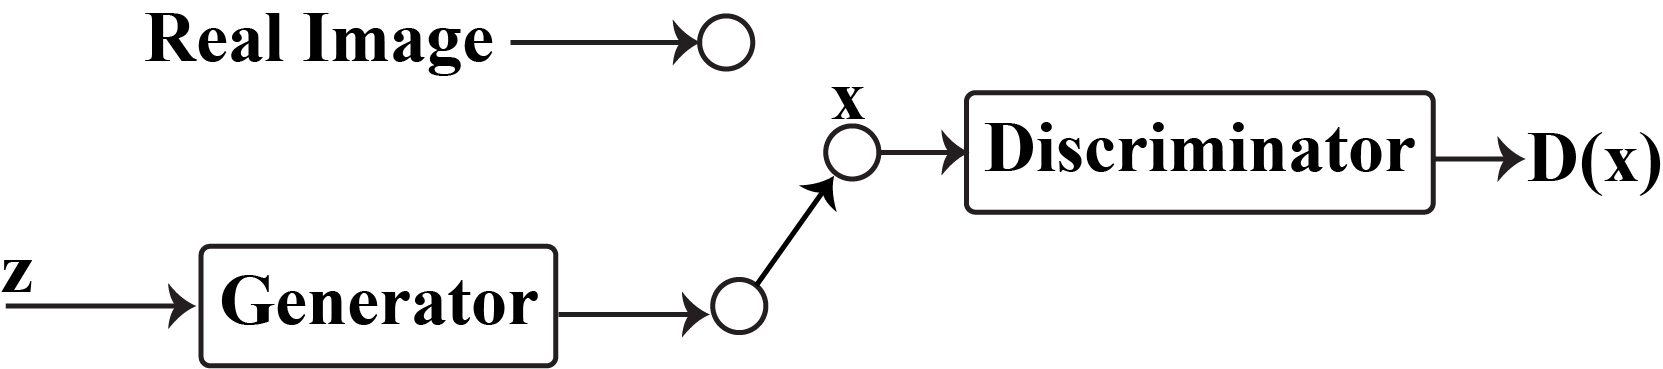
\includegraphics[width=\linewidth]{Training-Discriminator}}
\caption{Training Discriminator}
\label{fig}
\end{figure}

The discriminator generates a number $D(x)$ that represents the likelihood that x is a genuine data instance. Our goal is to increase the likelihood that created data instances will be identified as fake and actual data instances as real. i.e., the observed data's highest probability. Cost option uses cross entropy.

\begin{equation}
\begin{split}
\max \limits_{D} V(D) = & \mathbb{E}_{x\sim p_{data}(x)}[log D(x)] + \\& \mathbb{E}_{z\sim p_{z}(z)}[log (1-D(z))]
\end{split}
\end{equation}

%Training Generator
\subsubsection{Training Generator}\label{Training Generator}
With $D(x) = 1$, we want the generator to produce pictures. In other words, we train the generator to produce data instances that are inclined towards what the discriminator believes to be true by back propagating this target value all the way back to the generator.

\begin{figure}[h]
\centerline{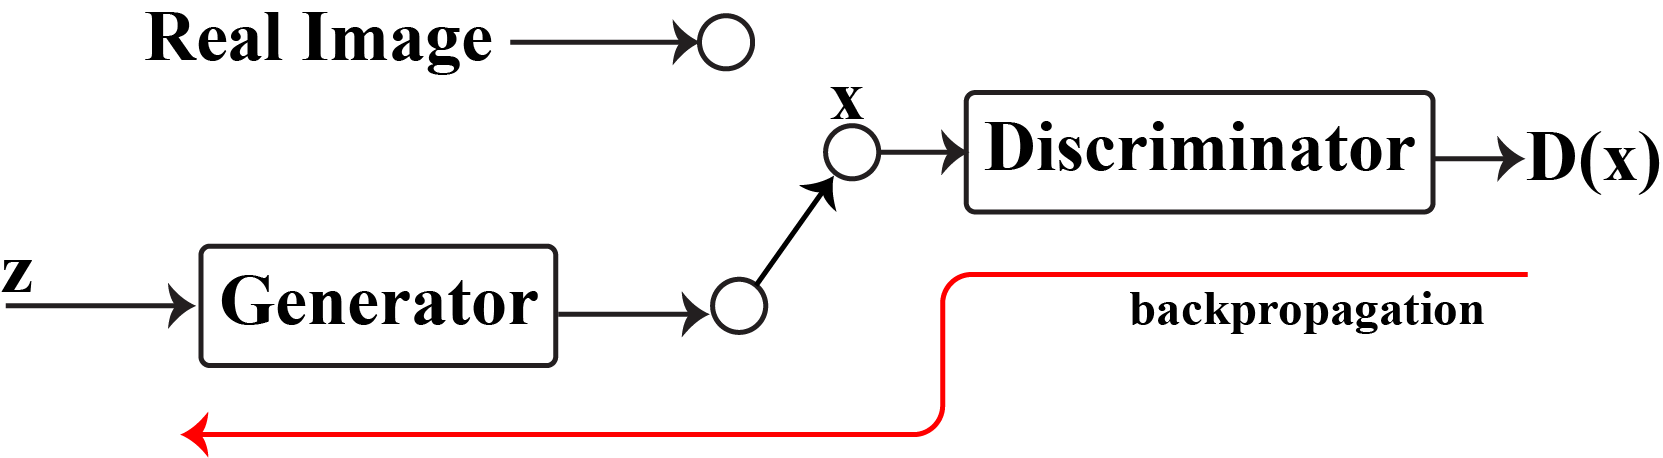
\includegraphics[width=\linewidth]{Training-Generator}}
\caption{Training Generator}
\label{fig}
\end{figure}

In order to trick the discriminator, the model's goal function on the generator side wants it to produce pictures with the highest $D(x)$ value.

\begin{equation}
\max \limits_{G} V(G) = \mathbb{E}_{z\sim p_{z}(z)}[log(1 - D(G(z)))]
\end{equation}

%Simultaneous Training Of Generator And Discriminator
\subsubsection{Simultaneous Training Of Generator And Discriminator}\label{Simultaneous Training Of Generator And Discriminator}
The alternating gradient descent is used to jointly learn the two goal functions after they have been specified. We fix the parameters of the generator model and do a single gradient descent iteration on the discriminator using the produced and real pictures. Next, we exchange positions. Resolve the discriminator issue and prepare the generator for one more iteration. As soon as the generator starts producing high-quality pictures, we alternate between training the two networks.

\begin{figure}[h]
\centerline{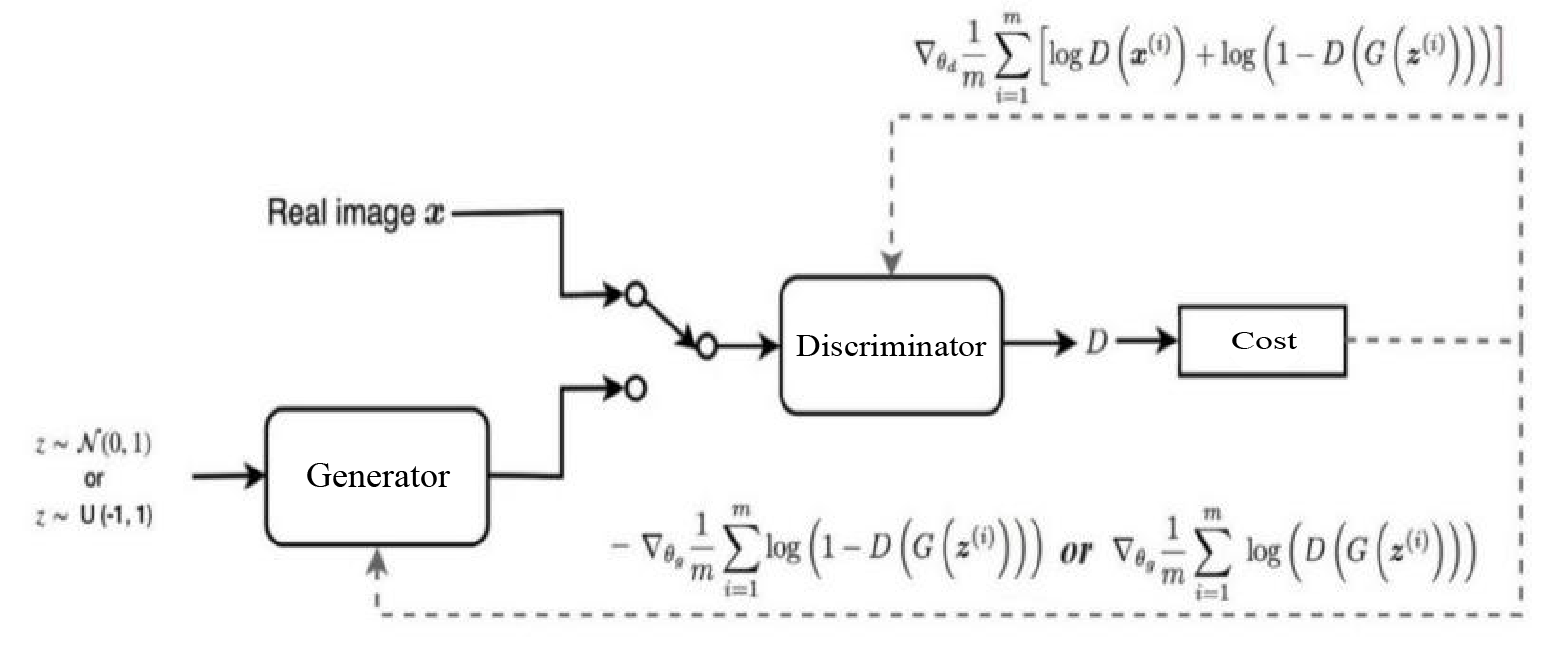
\includegraphics[width=\linewidth]{Traning-GAN}}
\caption{Training GAN}
\label{fig}
\end{figure}

%GAN for Image Colorization
\subsection{GAN for Image Colorization}\label{GAN for Image Colorization}
In GANs, a randomly produced noise vector serves as the generator network's input. However, in the job of picture colorization, such GANs won't be effective since our GAN isn't made to create images out of random vectors; rather, it's made to add colours to already-existing images that only have one channel (black and white). Therefore, adding three channels (RGB) with appropriate intensities for each colour channel is the fundamental challenge for our GAN. Therefore, to solve this issue, we employ Conditional GANs, a specific variety of GAN that takes as input grayscale pictures (with one intensity channel, or G(0 z |x) technically). To work with the GANs, the discriminator input is also altered. With the aforementioned revisions, our final cost functions are as follows.

\begin{equation}
\begin{split}
\min \limits_{\theta_{G}} J^{(G)}(\theta_{D},\theta_{G}) = \min \limits_{\theta_{G}}&-\mathbb{E}_z[log(D(G(0_z|x)))]+ \\& \lambda\parallel G(0_z|x)-y\parallel 1
\end{split}
\end{equation}
\begin{equation}
\begin{split}
\max \limits_{\theta_{G}} J^{(D)}(\theta_{D},\theta_{G}) =  \max \limits_{\theta_{D}}&(\mathbb{E}_y[log(D(y|x))]+ \\& \mathbb{E}_z[log(1-D(G(0_x|x)|x))])
\end{split}
\end{equation}
Grayscale image and produced image, as well as grayscale image and original picture, are the two inputs that the discriminator accepts. Then it decides if the couple is phoney or real.

%Method
\subsubsection{Method}\label{Method}
Our issue falls under the umbrella of image-to-image translation with mapping from high-dimension input to high-dimension output. It is really regression at the pixel level with the requirement that the output structure resemble the input structure. Therefore, the network must have very high spatial similarity between input and output, as well as providing information on each pixel's colour in the original grayscale image.

%GAN Architecture
\subsubsection{GAN Architecture}\label{GAN Architecture}
This model's network is built using "fully connected networks". In Generator, we employ layers of convolutions. However, downsampling the picture until it becomes a vector with a $2*2$ pixel size is done instead of pooling layers. The compressed portion is then expanded via upsampling to reach the input sample size $(32*32)$pixels. This tactic is inspired by specialised deep learning models called encoder-decoder networks, which comprise encoding and decoding networks for compressing and then extending the input and, as a result, reconstructing it. This method assists in network training without using a lot of memory. 

The input X for the generator is a grayscale picture with the size $(32*32*1)$. It is originally reduced in size using a kernel and stride of $1$ and $1$. Following this layer, it is compressed to an image of size $(2*2)$ using a kernel with stride size of $2$. After the first layer, this is repeated four more times to create the matrix with the dimensions $(2*2*512)$. 

Upsampling the matrix with kernel size $2$ and strides $2$ is what makes up the expansion stages, with the exception of the last layer. The structural integrity of the image is preserved by concatenating the $i$ and $n-i$ layers. To introduce noise for a robust training of the Generator, dropout of scale $0.5$ is used in the first and second expanding layers. For improved training, batch normalisation is used. LeakyReLU with a slope of $0.2$ was employed in our model since it performed better than ReLU activation function. Convolution with a kernel size of $1$ and a stride of $1$ is performed in the last layer to create an image with the dimensions $(32*32*3)$. Since "$\tanh$" activation function has demonstrated to perform better than linear activation functions, it is employed. It gives output in the form of matrix containing values from $-1$ to $1$. 
To minimise the cosine difference between the anticipated and the original picture, we train the model.

In order to create the coloured picture for the discriminator, we first concatenate the predicted or ground truth image in grayscale with the channel axis $($axis$=3)$. Using a convolutional layer with a filter size of $(2*2)$ and strides of $2$, we downscale the matrix sequentially. Each layer features a Leaky ReLU activation function with a slope of $0.2$, and each layer also undergoes batch normalisation. The final layer is flattened after which a hidden layer with $128$ units is linked to an output layer with one unit. The last layer uses a "sigmoid" activation function, which indicates the likelihood that the input picture belongs to the predicted one or the ground truth.

\begin{center}
$c1 -> [32,32,1] -> [32,32,64]$ \\
$c2 -> [32,32,64] -> [16,16,128]$ \\
$c3 -> [16,16,128] -> [8,8,256]$ \\
$c4 -> [8,8,256] -> [4,4,512]$ \\
$c5 -> [4,4,512] -> [2,2,512]$ \\
$DC0 -> [2,2,512] -> [4,4,512]$ \\
$DC1 -> [4,4,512] -> [8,8,256]$ \\
$DC2 -> [8,8,256] -> [16,16,128]$ \\
$DC3 -> [16,16,128] -> [32,32,64]$ \\
$DC4 -> [32,32,64] -> [32,32,3]$ \\
\text{Generator Architecture Plan}
\end{center}

\begin{center}
$c1 -> [32,32,ch] -> [16,16,64]$ \\
$c2 -> [16,16,64] -> [8,8,128]$ \\
$c3 -> [8,8,128] -> [4,4,256]$ \\
$c4 -> [4,4,256] -> [4,4,512]$ \\
\text{Discriminator Architecture Plan}
\end{center}

%Results
\section{Results}\label{Results}
The single channelled picture (also known as a grayscale image) is seen in the top image.
The picture produced by our GAN is seen in the centre image.
The reality is depicted in the bottom image.

\begin{figure}[h]
\centerline{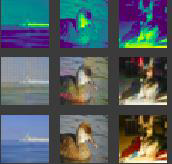
\includegraphics{res1}}
\label{fig}
\end{figure}
\begin{figure}[h]
\centerline{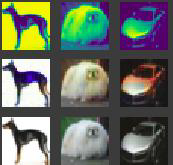
\includegraphics{res2}}
\label{fig}
\end{figure}
\begin{figure}[h]
\centerline{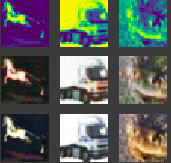
\includegraphics{res3}}
\label{fig}
\end{figure}
\begin{figure}[h]
\centerline{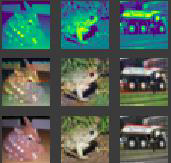
\includegraphics{res4}}
\caption{Results}
\label{fig}
\end{figure}

In this study, black and white photos were coloured using conditional GAN. While putting our research into practise, we came to the conclusion that the design of a neural network and the precise selection of hyperparameters serve as a bottleneck to the success of any deep learning project. We came to understand that even little adjustments to these features of the GAN can have a significant impact on the performance of the GAN or any neural network in general.we were successful in employing generative adversarial networks to automatically colour the grayscale photographs to a visually acceptable level. The synthetically coloured photos of CYPHER 10 created by GAN appeared to be pretty accurate replicas of the original photographs. During the training process, the model occasionally mistook sea water for grass, but with further practise, it was able to accurately colour vegetation in a green hue. In contrast to other colours, the model encountered particular problems with red, which it only learned after several epochs.


\begin{thebibliography}{00}

\bibitem{b1} Sankar, Rahul, et al. "Image Colorization Using GANs and Perceptual Loss." 2020 International Conference on Artificial Intelligence and Signal Processing (AISP). IEEE, 2020.

\bibitem{b2} He, Xinyu, Yikun Lu, and Yuxin Yang. "Colorization of Anime Gray Images via Generative Adversarial Networks." 2021 IEEE International Conference on Computer Science, Electronic Information Engineering and Intelligent Control Technology (CEI). IEEE, 2021.

\bibitem{b3} Ashwini, K., Rahul Reddy Pasham, and M. D. Sameer. "Coloring an Image Using Generative Adversarial Networks (GAN)." 2022 IEEE International Conference on Distributed Computing and Electrical Circuits and Electronics (ICDCECE). IEEE, 2022.

\bibitem{b4} Ashwini, K., Rahul Reddy Pasham, and M. D. Sameer. "Coloring an Image Using Generative Adversarial Networks (GAN)." 2022 IEEE International Conference on Distributed Computing and Electrical Circuits and Electronics (ICDCECE). IEEE, 2022.

\bibitem{b5} Le-Tien, Thuong, et al. "GAN-based Thermal Infrared Image Colorization for Enhancing Object Identification." 2021 International Symposium on Electrical and Electronics Engineering (ISEE). IEEE, 2021.

\bibitem{b6} Chai, Xinning, et al. "MLS-GAN: Multi-Level Semantic Guided Image Colorization." 2022 IEEE International Conference on Image Processing (ICIP). IEEE, 2022.

\bibitem{b7} Wu, Min, et al. "Remote sensing image colorization based on multiscale SEnet GAN." 2019 12th International Congress on Image and Signal Processing, BioMedical Engineering and Informatics (CISP-BMEI). IEEE, 2019.

\bibitem{b8} Wang, Yuyang, et al. "A Review of Gray-scale Image Recoloring Methods With Neural Network Based Model." 2022 7th International Conference on Image, Vision and Computing (ICIVC). IEEE, 2022.

\bibitem{b9} Nazeri, Kamyar, Eric Ng, and Mehran Ebrahimi. "Image colorization using generative adversarial networks." Articulated Motion and Deformable Objects: 10th International Conference, AMDO 2018, Palma de Mallorca, Spain, July 12-13, 2018, Proceedings 10. Springer International Publishing, 2018.

\bibitem{b10} Anwar, Saeed, et al. "Image colorization: A survey and dataset." arXiv preprint arXiv:2008.10774 (2020).

\bibitem{b11} Žeger, Ivana, et al. "Grayscale image colorization methods: Overview and evaluation." IEEE Access 9 (2021): 113326-113346.

\bibitem{b12} Nazeri, Kamyar, Eric Ng, and Mehran Ebrahimi. "Image colorization using generative adversarial networks." Articulated Motion and Deformable Objects: 10th International Conference, AMDO 2018, Palma de Mallorca, Spain, July 12-13, 2018, Proceedings 10. Springer International Publishing, 2018.

\bibitem{b13} Treneska, Sandra, et al. "GAN-Based image colorization for self-supervised visual feature learning." Sensors 22.4 (2022): 1599.

\bibitem{b14} Fu, Qiwen, Wei-Ting Hsu, and Mu-Heng Yang. "Colorization using convnet and gan." in Stanford University (2017): 1-8.

\bibitem{b15} Chen, Shu-Yu, et al. "A review of image and video colorization: From analogies to deep learning." Visual Informatics (2022).

\bibitem{b16} Suárez, Patricia L., Angel D. Sappa, and Boris X. Vintimilla. "Infrared image colorization based on a triplet dcgan architecture." Proceedings of the IEEE Conference on Computer Vision and Pattern Recognition Workshops. 2017.

\end{thebibliography}




\end{document}
